\subsection*{Problem 6: LQR Output Feedback Regulation (Full Order)}
\subsubsection*{a) Design the observer for the linear model.}


Given LQR is a form of control, not much changed when designing the Output Feedback Observer. In fact, the same methodology from Project 1 was used to design the observer. The same LQR controller from Problem 3 was used and the closed-looped eigenvalues of that controller were multiplied by 7.5 to be used in designing the observer. These new scaled eigenvalues were used in the \codeword{place()} function in MATLAB to get the following observer gains:

\begin{equation*}
    \begin{split}
        L & =
        \begin{bmatrix}
            73.95  & -6.51   \\
            719.20 & -226.84 \\
            2.66   & 37.18   \\
            268.62 & 289.14  \\
        \end{bmatrix}
    \end{split}
\end{equation*}

The closed-loop eigenvalues are found from $det(sI-(A-LC))=0$. They are the following:

\begin{equation*}
    \begin{split}
        s & = -9.91\pm6.60, -28.90, -62.59
    \end{split}
\end{equation*}

This design satisfies the requirements still as we can perfectly observe the output states with fast enough eigenvalues given there is no noise in our measurements.

The following figures depict the outputs and input of the linear system with the above controller:

\begin{figure}[!ht]
    \centering
    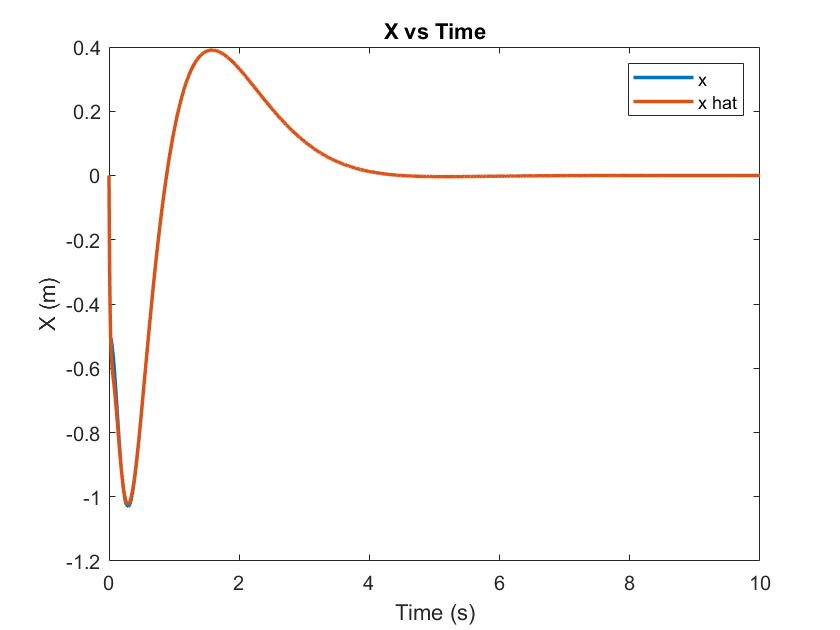
\includegraphics[width=\linewidth]{figs/of_lin_x.png}
    \caption{Linear System X Output}
    \label{}
\end{figure}

\begin{figure}[!ht]
    \centering
    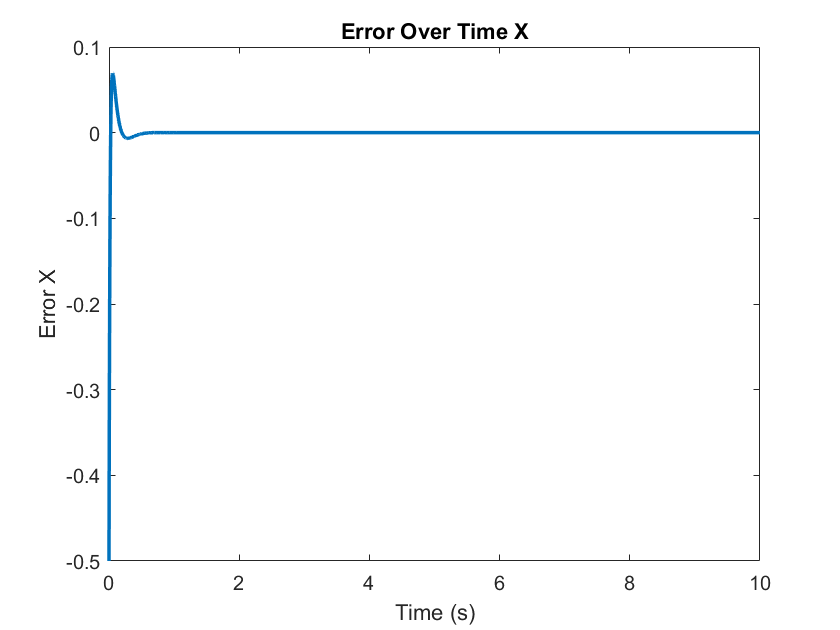
\includegraphics[width=\linewidth]{figs/of_lin_x_err.png}
    \caption{Linear System X Error}
    \label{}
\end{figure}

\begin{figure}[!ht]
    \centering
    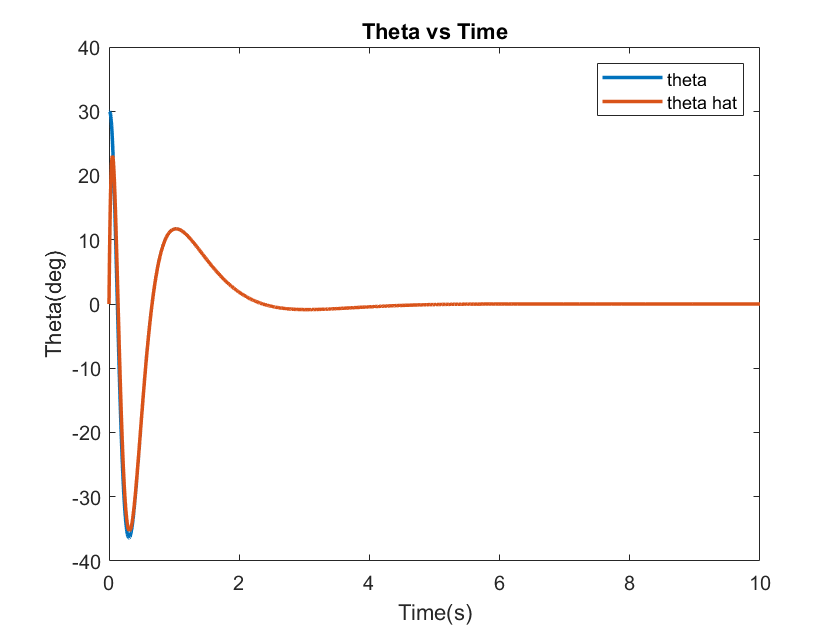
\includegraphics[width=\linewidth]{figs/of_lin_theta.png}
    \caption{Linear System $\theta$ Output}
    \label{}
\end{figure}

\begin{figure}[!ht]
    \centering
    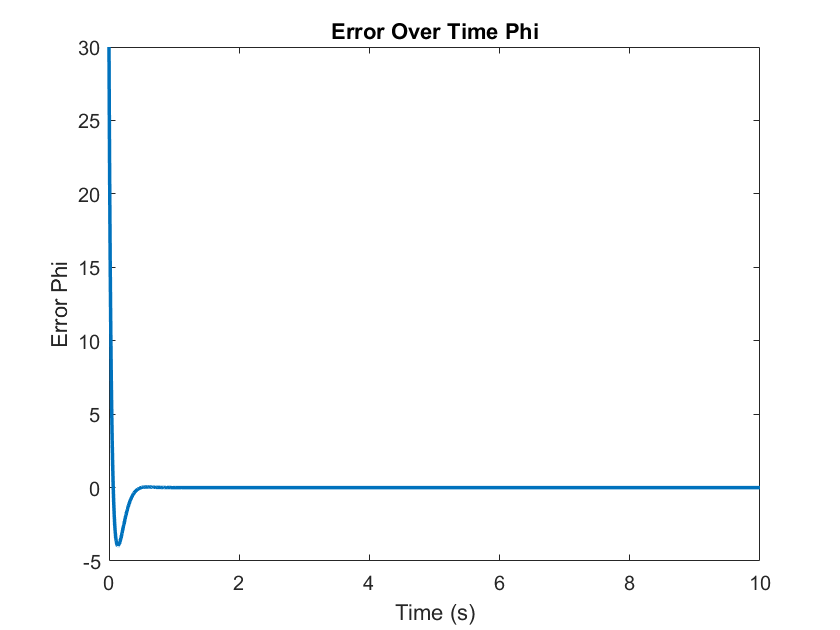
\includegraphics[width=\linewidth]{figs/of_lin_theta_err.png}
    \caption{Linear System $\theta$ Error Input}
    \label{}
\end{figure}


\begin{figure}[!ht]
    \centering
    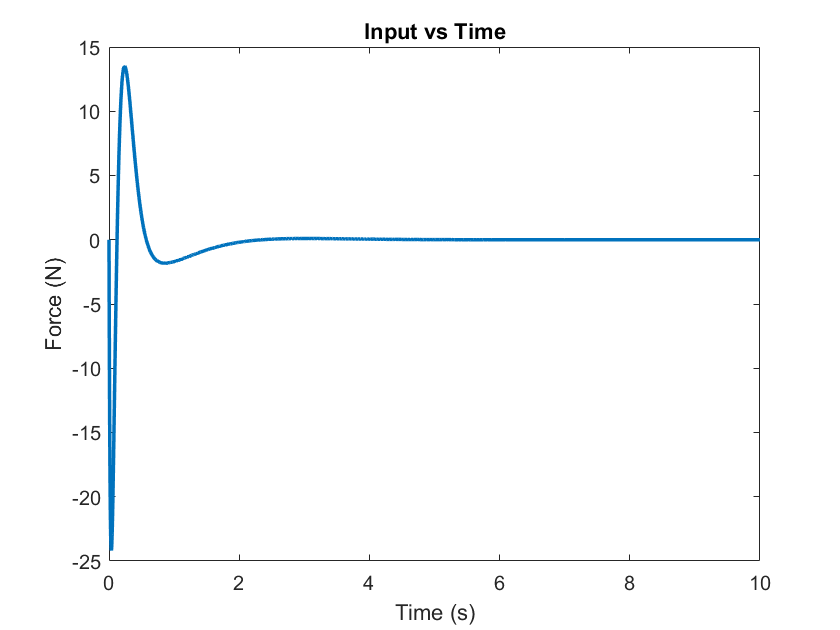
\includegraphics[width=\linewidth]{figs/of_lin_input.png}
    \caption{Linear System Input}
    \label{}
\end{figure}

\clearpage

\subsubsection*{b) Design the observer for the nonlinear model.}

The controller and observer used for the nonlinear system are the same as for the linear model. There is enough design buffer to compensate for the nonlinear dynamics much like in Problem 3. The closed-loop eigenvalues are found from $det(sI-(A-LC))=0$ and are the same as the linear model. They are the following:

\begin{equation*}
    \begin{split}
        s & = -9.91\pm6.60, -28.90, -62.59
    \end{split}
\end{equation*}

The eigenvalues of $A-BK$ are the same as Problem 3 given the controller didn't change. They are the following:

\begin{equation*}
    \begin{split}
        s & = -1.32\pm0.88, -3.85, -8.34
    \end{split}
\end{equation*}

The following figures depict the outputs and input of the nonlinear system with the above controller:

\begin{figure}[!ht]
    \centering
    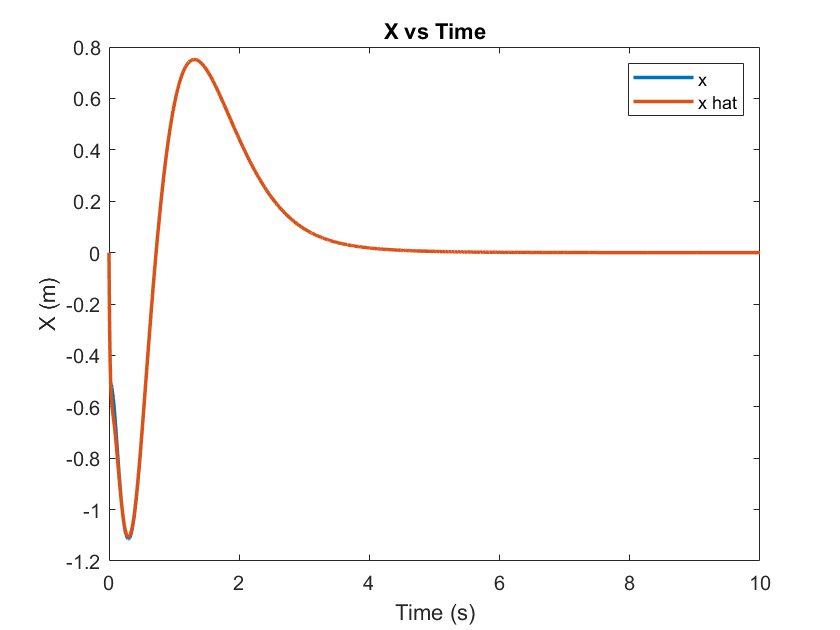
\includegraphics[width=\linewidth]{figs/of_nlin_x.png}
    \caption{Nonlinear System X Output}
    \label{}
\end{figure}

\begin{figure}[!ht]
    \centering
    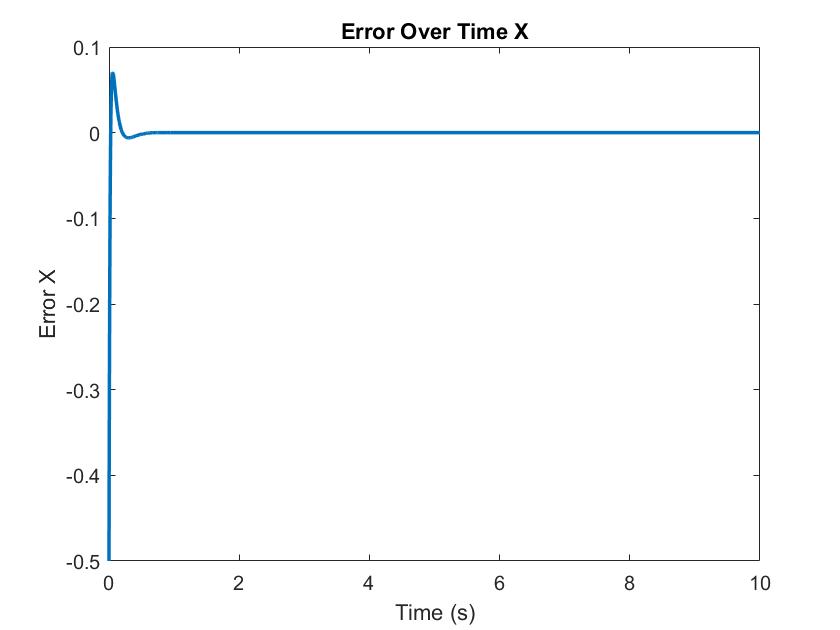
\includegraphics[width=\linewidth]{figs/of_nlin_x_err.png}
    \caption{Nonlinear System X Error}
    \label{}
\end{figure}

\begin{figure}[!ht]
    \centering
    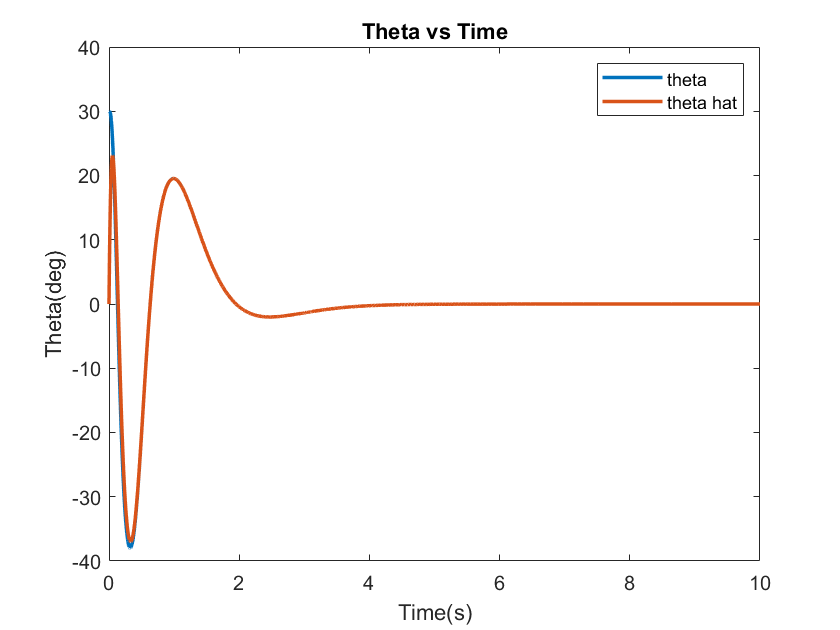
\includegraphics[width=\linewidth]{figs/of_nlin_theta.png}
    \caption{Nonlinear System $\theta$ Output}
    \label{}
\end{figure}

\begin{figure}[!ht]
    \centering
    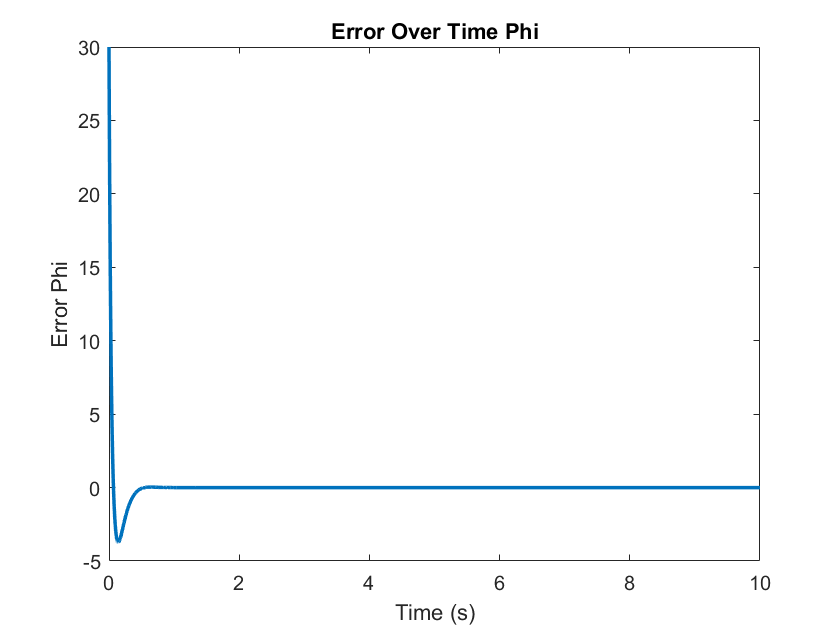
\includegraphics[width=\linewidth]{figs/of_nlin_theta_err.png}
    \caption{Nonlinear System $\theta$ Error Input}
    \label{}
\end{figure}


\begin{figure}[!ht]
    \centering
    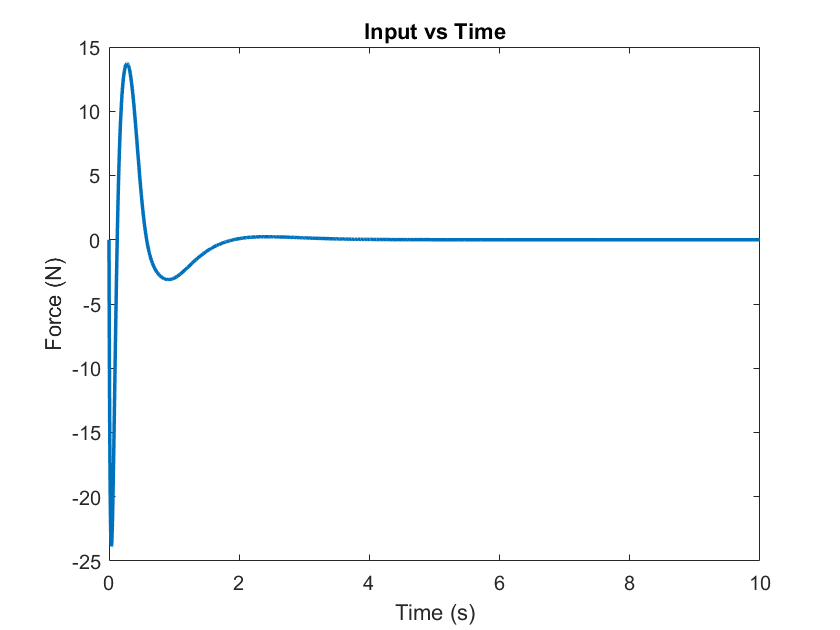
\includegraphics[width=\linewidth]{figs/of_nlin_input.png}
    \caption{Nonlinear System Input}
    \label{}
\end{figure}

\clearpage

\subsubsection*{c) Compare the responses of the system under state feedback to the responses of the system under
    output feedback. }

The outputs for each of these cases look relatively similar as there is no noise on the ``measurements” we’re using in our observer. The transient responses for each look slightly different on a small scale until the observer tracks with zero error; however, it is hard to notice the difference in the transients graphically. Once tracking, the responses look the same as the controller eigenvalues are the same for state and output feedback. This is the case for the linear and nonlinear models where the only difference is the slightly slower response in the nonlinear case.